\documentclass{article}

\usepackage{lastpage} % for the number of the last page in the document
\usepackage{fancyhdr}
\usepackage{geometry}
\usepackage{graphicx}
\usepackage{grffile}
\usepackage[utf8x]{inputenc}
\geometry{a4paper}
\geometry{portrait}
\pagestyle{fancy}
\usepackage{float}
\fancyhf{}
\lhead{KinderFinder - Testing Information}
\rhead{Section \thesection}
\lfoot{}
\rfoot{Page \thepage\ of \pageref{LastPage}}


%\begin{figure}[H]
%\centering
%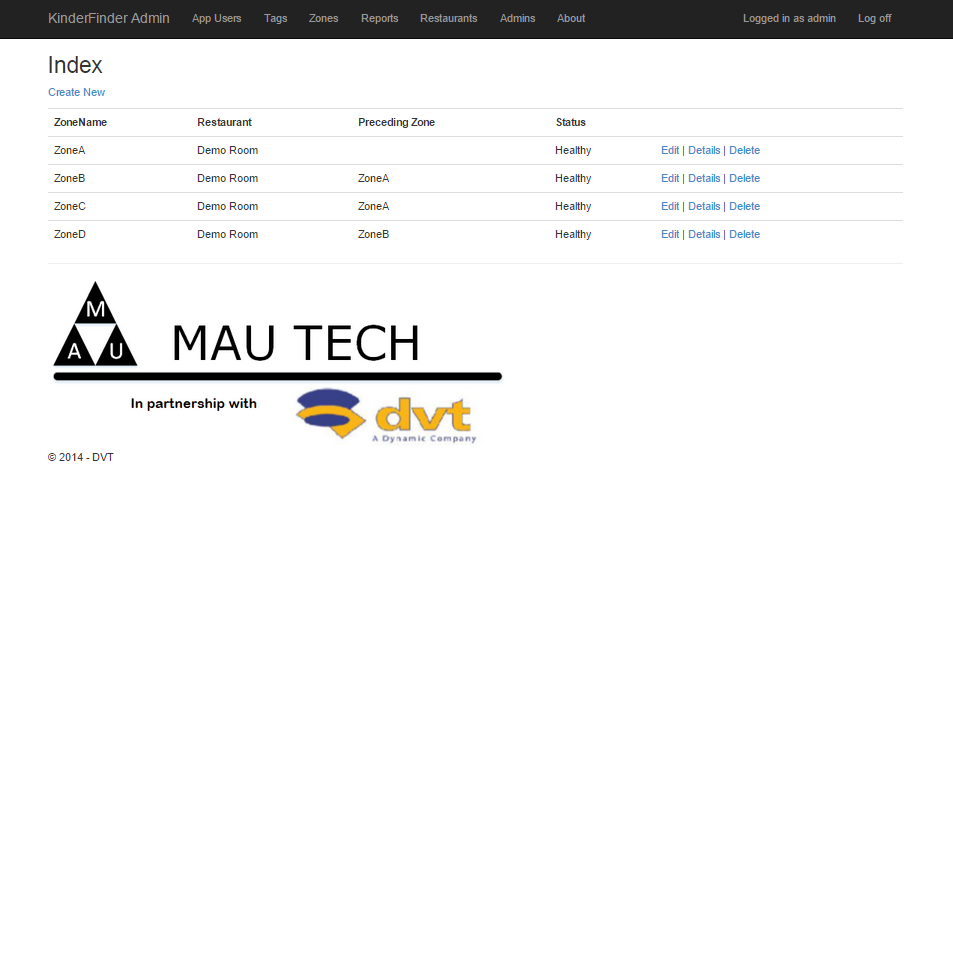
\includegraphics[scale=0.5]{adminportalzones.png}
%\caption{Use case of Android app user (first level granularity).}
%\end{figure}

\newcommand{\horrule}[1]{\rule{\linewidth}{#1}}

\title{
		\normalfont \normalsize \textsc{Client Name: DVT} \\
		\normalfont \normalsize \textsc{Project Name: KinderFinder} \\ [25pt]
		\horrule{0.5pt} \\[0.4cm]
		\huge KinderFinder Testing Information \\
		\horrule{2pt} \\[0.5cm]
}
\author{\begin{tabular}{rl}
	\texttt{Team Name:} & \texttt{MAU Technologies} \\[0.5cm]
	Uteshlen Nadesan & 28163304 \\
	Michael Johnston & 12053300 \\
	Po-Han Chiu & 11063612
\end{tabular}
	\\ \\ \texttt{}
	\\ \\ \texttt{Version: 1}}
\date{20 October 2014} 


\begin{document}
\maketitle
\newpage

\tableofcontents
\newpage

%%%unit testing (test in isolation with mocking)
%- how tests can be executed (e.g. via Maven)
%- how the tests were developed
%- the tests coverage (% functionality tested)
%%%integration testing (test complete system)
%%%non-functional testing (performance, security etc.)
%%%usability testing (if any, process + results)

\section{Quality Assurance}
\paragraph{}Our quality management is done and incorporated into our software development and project management process.

\paragraph{}During the development process of this project, we have constantly updated our documentation of the requirements for this project. We immediately make the changes on our documentation whenever a change occurs or a better way of implementation of the software is found during development.

\paragraph{}We make sure that we have achieved what we have documented and adhere to the requirements of our client, and inform our clients if a change to the requirements when necessay.

\section{Testing}
Testing is done at every stage of our software development. This ensures that our code are of consistent quality. Our testing processes are repeatable, this allows us to measure performance, quality and output results.

\subsection{Unit Testing}
\paragraph{}We test every function that we code immediately after we have written it. This way, when we code another function that is dependant on a function we have previously written, we can be assured that any bugs that occur are from the function we are currently working with. This allows us to reduce the scope of our search of the bug, and reduces our time looking for the bug in the long term of development.

\paragraph{}The technique we use for unit tests are generally manual testing. We manually add mock data as input and then look at the output to see if it is the same as we expected.

\paragraph{}We have covered most of the test cases that we can think of, the test coverage can be estimated to be around 90\%. We leave the last 10\% for the cases that we have never thought of.






\end{document}
